% CSE440 Lab Project — ACL-style research report
% Paste this file (and custom.bib, and the figures/ folder) into the official
% ACL LaTeX template project on Overleaf:
% https://www.overleaf.com/latex/templates/association-for-computational-linguistics-acl-conference/jvxskxpnznfj
% Replace the template's main.tex with this file and its custom.bib with this one.
%
% %TODO markers throughout mark content that depends on work not yet executed
% (see the project's PROJECT_CONTEXT.md, Sections 9.6 and 11 for the exact list).

\documentclass[11pt]{acl}

\usepackage[T1]{fontenc}
\usepackage[utf8]{inputenc}
\usepackage{microtype}
\usepackage{inconsolata}
\usepackage{times}
\usepackage{latexsym}
\usepackage{graphicx}
\usepackage{booktabs}
\usepackage{multirow}
\usepackage{amsmath}
\usepackage{amssymb}
\usepackage{xcolor}

\newcommand{\todo}[1]{\textcolor{red}{\textbf{[TODO: #1]}}}

% %TODO: replace with the real title if the team prefers a different framing.
\title{Leakage-Aware Privacy Practice Classification: A Comparative Study of\\
Classical and Neural Models under Policy-Disjoint Evaluation}

% %TODO: replace with real author names, student IDs, and affiliation details
% before submission (naming convention: GroupNo\_ID1\_ID2\_ID3\_ID4).
\author{
Author One$^{1}$ \quad Author Two$^{1}$ \quad Author Three$^{1}$ \quad Author Four$^{1}$ \\
$^{1}$Department of Computer Science and Engineering, BRAC University \\
\texttt{\{student.id1, student.id2, student.id3, student.id4\}@g.bracu.ac.bd}
}

\begin{document}
\maketitle

\begin{abstract}
Privacy policies are long, legally dense documents that almost nobody reads in full,
yet they govern how personal data is collected, shared, and retained. We study
automatic classification of privacy-policy clauses into eight standardized data-practice
categories defined by the OPP-115 corpus, framing the task as single-label,
multi-class text classification of an annotated span with its surrounding clause
available as context. Beyond the required comparison of classical and neural
architectures, our central methodological contribution is a systematic evaluation of
\emph{train/test leakage}: because privacy policies reuse boilerplate legal language
across otherwise unrelated documents, a conventional row-level stratified split allows
the same policy, and the same boilerplate phrasing, to appear in both training and test
data. We construct and report results under two split schemes -- a leaky, row-level
\texttt{random} split and a \texttt{policy}-disjoint split that holds out entire policies
-- and evaluate three classical machine learning models (Random Forest, Logistic
Regression, Naive Bayes) and seven neural architectures (SimpleRNN, GRU, LSTM, and their
bidirectional variants, plus a fine-tuned BERT Base) under both. Evaluating on the leaky
split inflates macro-F1 by 0.015--0.123 depending on model, and \emph{changes which model
appears best} -- the model with the highest accuracy under the leaky split is, in one
case, the worst-generalizing model of all ten trained. Under the honest, policy-disjoint
evaluation, a resource-constrained fine-tune of BERT Base attains the best macro-F1
(0.7060), narrowly ahead of a tuned Naive Bayes classifier (0.7011), while showing the
smallest leakage-driven inflation of any model -- evidence that its advantage comes from
pretraining rather than memorizing this corpus's specific boilerplate. We frame this
leakage-aware protocol as this paper's central, deliberately scoped novelty claim, and
draw an explicit boundary around three brainstormed extensions -- context-aware span
+ clause modeling, minority-class-aware training, and a cross-market external-validation
study on non-US privacy policies -- that we designed but placed out of scope for this
paper, reporting them here only as future work.
\end{abstract}

\section{Introduction}
\label{sec:intro}

Privacy policies are the primary legal instrument through which organizations disclose
how they collect, use, share, and retain personal data. In practice they are long,
formulaically written, and inconsistently structured, and empirical studies have long
noted that almost no user reads them in full before consenting. Automatically mapping
policy text onto a standardized taxonomy of data practices -- what data is collected, by
whom, whether it is shared with third parties, what choices a user has, how long it is
retained -- would let downstream tools summarize a policy at a glance, flag practices
relevant to a specific regulation (e.g.\ GDPR or CCPA), or let researchers compare
practices across companies and over time at corpus scale. This is squarely a
multi-class text classification problem, and unlike sentiment analysis or movie
recommendation it is not a solved, saturated task: privacy language is technical, class
frequencies are heavily skewed toward a small number of common practices, and a single
clause frequently expresses more than one practice at once.

We build our study on the OPP-115 corpus \cite{wilson-etal-2016-creation}, 115 real-world
website privacy policies manually annotated by legal experts against a fixed schema of
data-practice categories. Following the corpus's own annotation unit, we treat each
annotated \emph{span} -- the exact stretch of text an annotator highlighted as evidence
of a practice -- as one classification instance, labeled with one of eight practice
categories, with the full clause that contains the span available as additional context.
Reported in preliminary analysis of the working dataset built from this corpus (17,343
labeled spans across 115 policies), two structural properties of the data directly shape
our experimental design and are elaborated in Section~\ref{sec:dataset}: an
approximately 24$\times$ imbalance between the largest and smallest category, and a
substantial fraction of underlying clauses that legitimately carry more than one
category simultaneously.

A third, less obvious property motivates this paper's central methodological
contribution. Privacy policies reuse legally vetted boilerplate language across
otherwise unrelated organizations -- template clauses drafted by the same law firm or
copied from a common source frequently recur, word for word, across dozens of policies.
This means that rows in a policy-clause dataset are not independent draws: many rows
share a parent clause, many clauses share a parent policy, and many policies share
literal boilerplate text with other policies. A conventional \emph{row-level} stratified
train/test split -- the default choice in most classification pipelines, including the
course's own reference materials -- ignores this structure and can place near-identical
boilerplate text on both sides of the split. A model can then score well by recognizing
a specific policy or phrase it has already memorized rather than by learning what
privacy language of a given category actually looks like. This is a specific instance
of a broader, well-documented problem in NLP evaluation: standard splits and
benchmark reuse can silently overstate a model's real generalization ability
\cite{gorman-bedrick-2019-need,lewis-etal-2021-question}.

We therefore evaluate every model under two split schemes, constructed identically for
every model to keep the comparison fair: a \texttt{random} row-level stratified split
(the leaky, optimistic condition a conventional pipeline would produce) and a
\texttt{policy}-disjoint split that holds every row of a given policy entirely within one
of train, validation, or test. Reported in preliminary analysis, the gap between these
two conditions is itself the paper's headline finding, not an artifact to be hidden: it
is large, it is architecture-dependent, and it changes which model a project would ship
if it evaluated only on the conventional split. We combine this leakage-aware evaluation
with the course's required breadth of models -- three classical machine learning
baselines and seven neural architectures spanning recurrent networks and a fine-tuned
transformer -- to produce, to our knowledge, the first systematic comparison of how
susceptible different model families are to boilerplate memorization on this task.

Our contributions are: (1) a leakage-aware evaluation protocol for privacy-policy
classification, contrasting a conventional row-level split against a policy-disjoint
split across ten models spanning four architecture families; (2) an empirical finding
that leakage-driven score inflation is highly non-uniform across architectures and
correlates with how much of a model's representational capacity was fit on this
dataset's own boilerplate rather than external data; and (3) a full implementation and
comparison of the classical and neural model suite required for privacy-practice
classification on OPP-115, including a resource-constrained BERT Base fine-tune
practical on consumer hardware.

\paragraph{Scope of this paper's novelty.} Because the course specification explicitly
treats ``we compared several models'' and ``we used BERT'' as baseline requirements
rather than contributions, we state precisely what this paper does and does not claim.
Our brainstorming process considered a dozen candidate novelty directions for this
dataset, from leakage-aware evaluation and minority-class-aware training to span-versus-
clause context, cross-market external validation, and disclosure-risk scoring. Of
these, we implement and report exactly one -- leakage-aware, policy-disjoint evaluation
-- as this paper's sole methodological contribution, deliberately rather than by
omission: one rigorously executed, fully evaluated claim is more defensible within a
7--8 page report than several partially explored ones. Three closely related directions
were designed but are intentionally left \emph{out of this paper's scope}, reported only
as future work in Section~\ref{sec:conclusion}: (i) context-aware classification that
feeds the full clause alongside the annotated span, to test whether it disambiguates the
First-Party/Third-Party confusion identified in Section~\ref{sec:per-class}; (ii)
minority-class-aware training targeted at the one category where
Section~\ref{sec:per-class} shows scarcity, rather than semantic overlap, is the
bottleneck; and (iii) an external validation study applying this paper's trained
classifier to a different market of English-language privacy policies (a planned
Bangladesh-focused comparison) -- a genuinely separate research question reusing this
project's trained model rather than extending its evaluation protocol, not attempted
here.

\section{Related Work}
\label{sec:related}

\paragraph{Privacy policy analysis.} The OPP-115 corpus
\cite{wilson-etal-2016-creation} is the standard manually annotated benchmark for
data-practice classification in privacy policies and is the dataset used throughout this
work: 115 website privacy policies, each independently annotated by three annotators
against a fixed ten-category schema, later consolidated into agreed-upon labels. Building
on this resource, \citet{harkous-etal-2018-polisis} present Polisis, a deep-learning
pipeline that classifies privacy-policy segments into data-practice categories and
supports downstream question answering over the resulting structured representation,
establishing that neural sequence models can substantially outperform earlier
rule-based and shallow feature-based privacy-policy classifiers. Our work differs in
focus rather than in dataset: rather than proposing a new architecture for this task, we
hold the model suite close to what prior work and the course specification already
require, and instead study how the \emph{evaluation protocol itself} -- specifically,
how the train/test split respects or ignores document-level structure -- changes which
architecture appears to win.

\paragraph{Multi-class text classification.} The standard progression of methods for
multi-class text classification moves from sparse feature-based methods to learned
distributed representations to pretrained transformers. Bag-of-words representations
such as TF-IDF paired with linear or Bayesian classifiers remain strong, fast baselines
\cite{pedregosa-etal-2011-scikit}. Distributed word embeddings such as word2vec
\cite{mikolov-etal-2013-efficient} and GloVe \cite{pennington-etal-2014-glove} let
classifiers generalize across semantically related but lexically distinct terms.
Recurrent architectures -- Elman-style RNNs, their gated successors LSTM
\cite{hochreiter-schmidhuber-1997-lstm} and GRU \cite{cho-etal-2014-learning}, and their
bidirectional variants \cite{schuster-paliwal-1997-bidirectional} -- model sequential
and contextual dependencies that bag-of-words representations discard entirely.
Pretrained transformers, exemplified by BERT \cite{devlin-etal-2019-bert}, extend this
further by learning contextual representations from very large external corpora before
any task-specific fine-tuning. This project's model suite is deliberately designed to
span all four tiers of this progression on a single dataset and evaluation protocol,
which is what makes the leakage-inflation comparison in
Section~\ref{sec:results} interpretable across architecture families rather than
confounded by dataset or preprocessing differences.

\paragraph{Evaluation leakage and standard splits.} A growing body of NLP evaluation
literature argues that widely used ``standard'' splits and naively constructed
train/test partitions can systematically overstate generalization.
\citet{gorman-bedrick-2019-need} show that re-splitting standard NLP benchmarks and
re-running standard models changes both absolute scores and relative model rankings,
arguing that a single fixed split is an unreliable basis for claiming one model is
better than another. \citet{lewis-etal-2021-question} document a closely related but
more specific failure mode in open-domain question answering: substantial overlap
between training and test questions inflates reported accuracy and misrepresents how
well models generalize to genuinely novel inputs. Our work applies the same underlying
principle -- that a split must respect the natural grouping structure of the data --
to a domain where that structure is unusually explicit: privacy policies are grouped by
source document, and boilerplate legal language is reused verbatim across otherwise
unrelated documents, so a row-level split leaks not just topical similarity but literal,
identical text across the train/test boundary.

\paragraph{Class imbalance in text classification.} OPP-115's category distribution is
highly skewed (Section~\ref{sec:dataset}), a pattern common to many real-world text
classification corpora. \citet{johnson-khoshgoftaar-2019-survey} survey deep-learning
approaches to class imbalance and group mitigations into three families: data-level
resampling (oversampling minority classes, undersampling majority classes, or
synthetic techniques such as SMOTE), algorithm-level reweighting (class-weighted loss
functions, focal loss), and evaluation-level choices such as reporting macro-averaged
rather than micro-averaged metrics so that minority classes are not masked by overall
accuracy. This project adopts the third family throughout -- macro-F1 as the primary
metric and per-class precision/recall/F1 reported for every model -- and includes
class-weighted configurations in its hyperparameter grids (Section~\ref{sec:models}) as
an instance of the second family, consistent with the survey's recommendation that no
single mitigation is free and that its effect should be measured per class rather than
assumed.

\section{Methodology}
\label{sec:methodology}

\subsection{Dataset and Exploratory Data Analysis}
\label{sec:dataset}

\paragraph{Source and construction.} We use the OPP-115 corpus
\cite{wilson-etal-2016-creation}: 115 website privacy policies, each independently
annotated by three annotators against a fixed schema, later merged by the corpus's own
consolidation algorithm at a 0.75 overlap-similarity threshold. Reported in preliminary
analysis, this threshold reproduces the original corpus statistics most closely among
the thresholds shipped with the corpus, including an exact match on the 92/23 policy
train/test split. From each surviving annotated practice we take the longest populated
selected span as the classification input (\texttt{text}) and attach the full clause
containing that span as additional context (\texttt{clause\_text}), joined with policy
metadata. Two of the corpus's ten original categories, \emph{Other} (generic
introductory boilerplate, not a specific data practice) and \emph{Do Not Track} (very
low frequency, narrow scope), are dropped, leaving the eight categories used throughout
this paper: \emph{First Party Collection/Use}, \emph{Third Party Sharing/Collection},
\emph{User Choice/Control}, \emph{Data Security}, \emph{User Access, Edit and Deletion},
\emph{International and Specific Audiences}, \emph{Policy Change}, and \emph{Data
Retention}.

\paragraph{Scale.} Reported in preliminary analysis, the resulting working dataset
contains 17{,}343 labeled spans drawn from 3{,}204 distinct underlying clauses and 115
distinct policies, well above the course's 10{,}000-row minimum and comfortably above
the four-class minimum with eight classes. Annotated spans are short (mean 137
characters, approximately 22 words; median 92 characters), while the surrounding clauses
are substantially longer (mean 636 characters, approximately 101 words), which is why
the clause is retained only as optional context rather than as the primary classifier
input.

\paragraph{Class imbalance.} Figure~\ref{fig:class-dist} shows the category
distribution. \emph{First Party Collection/Use} and \emph{Third Party
Sharing/Collection} together account for 74.8\% of all rows, while the smallest
category, \emph{Data Retention}, accounts for only 1.9\% -- a 24.3$\times$ ratio between
the largest and smallest class. Reported in preliminary analysis, this imbalance is the
primary reason accuracy is never reported as a standalone metric anywhere in this paper
(Section~\ref{sec:results} shows a concrete case where the highest-accuracy model is the
worst model by macro-F1); every evaluation instead centers macro-F1 and reports full
per-class breakdowns.

\begin{figure}[t]
\centering
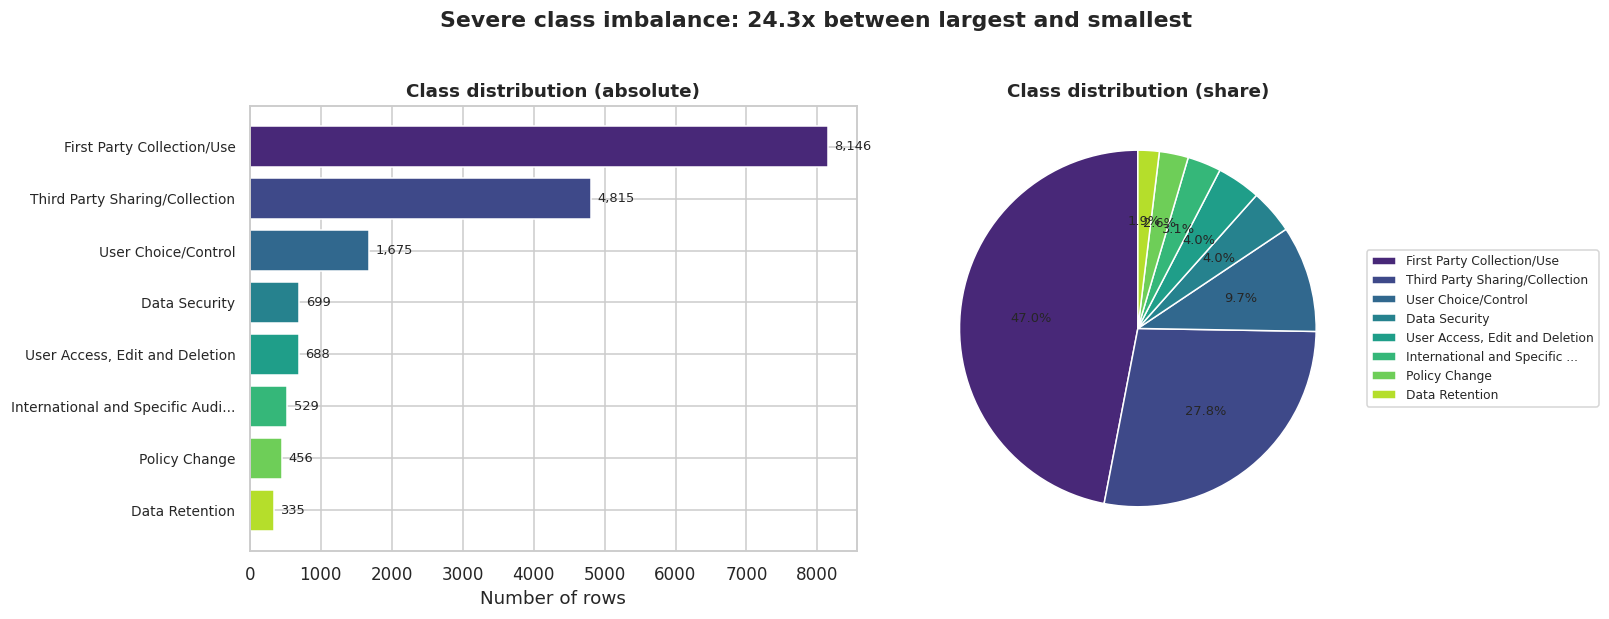
\includegraphics[width=\columnwidth]{figures/class_distribution.png}
\caption{Category distribution over the 17{,}343-row working dataset. The two most
frequent categories account for 74.8\% of all rows; the ratio between the largest and
smallest category is 24.3$\times$.}
\label{fig:class-dist}
\end{figure}

\paragraph{Span length.} Figure~\ref{fig:span-length} shows the distribution of span
length in words and characters. Most spans are short, single-sentence excerpts, with a
long right tail of longer selected passages (maximum 1{,}873 characters). This
distribution motivates the sequence-length cap used for the recurrent models
(Section~\ref{sec:models}): padding or truncating to 48 tokens covers the 92nd
percentile of span length while keeping training tractable.

\begin{figure}[t]
\centering
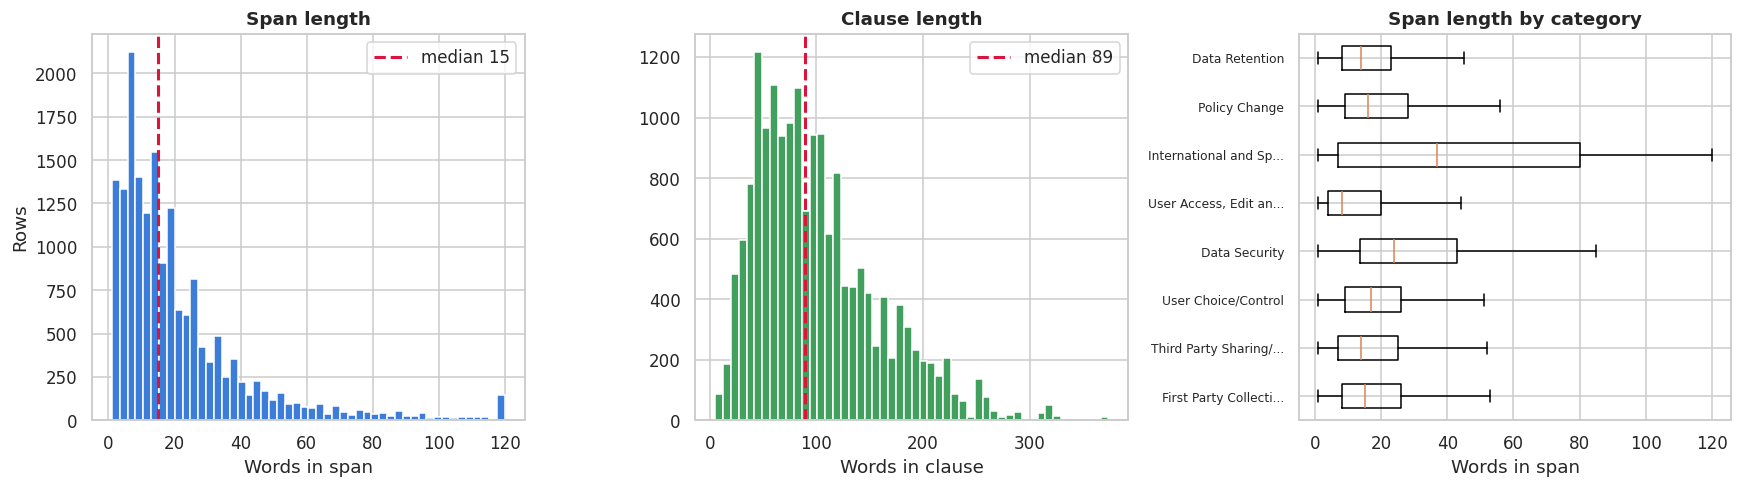
\includegraphics[width=\columnwidth]{figures/span_length.png}
\caption{Distribution of annotated-span length in words (left) and characters (right).
Dashed lines mark the median.}
\label{fig:span-length}
\end{figure}

\paragraph{Multi-practice clauses.} Reported in preliminary analysis, 1{,}119 of the
3{,}204 distinct underlying clauses (34.9\%) carry more than one category -- for
example, a single sentence such as \emph{``we collect your email address and may share
it with advertising partners unless you opt out''} simultaneously expresses \emph{First
Party Collection/Use}, \emph{Third Party Sharing/Collection}, and \emph{User
Choice/Control}. This finding is the reason the clause is never used as the sole
classification input in this project: a clause-level single-label formulation would
force a single label onto text that legitimately expresses several practices, and would
in any case yield only around 3{,}204 rows, short of the required minimum. The
annotated span, which an expert human annotator has already disambiguated to one
practice, is therefore the primary input, with the clause retained as optional context
for future context-aware modeling (Section~\ref{sec:conclusion}).

\paragraph{Boilerplate reuse and split structure.} Reported in preliminary analysis, even
under a policy-disjoint split, 233 test rows (6.0\%) share identical underlying clause
text with some row in the training policies -- real-world reuse of standard legal
language across unrelated organizations rather than a defect in the split. This is
categorically different from, and much smaller than, what a naive row-level split
produces: under the row-level \texttt{random} scheme used as the leaky comparison
condition in this paper, 113 of 115 policies appear on both sides of the split and
95.2\% of test rows share clause text with some training row. This gap -- 6.0\%
irreducible real-world reuse versus 95.2\% construction-induced leakage -- is the
concrete motivation for the dual-scheme evaluation protocol in
Section~\ref{sec:protocol}.

\paragraph{Word cloud.} Figure~\ref{fig:wordcloud} visualizes the most frequent terms
across all annotated spans after standard stopword removal, dominated by data-practice
vocabulary (\emph{information}, \emph{personal}, \emph{data}, \emph{use}, \emph{third
party}, \emph{may}) that is broadly shared across categories -- itself a preview of the
category-overlap difficulty discussed in Section~\ref{sec:results}.

\begin{figure}[t]
\centering
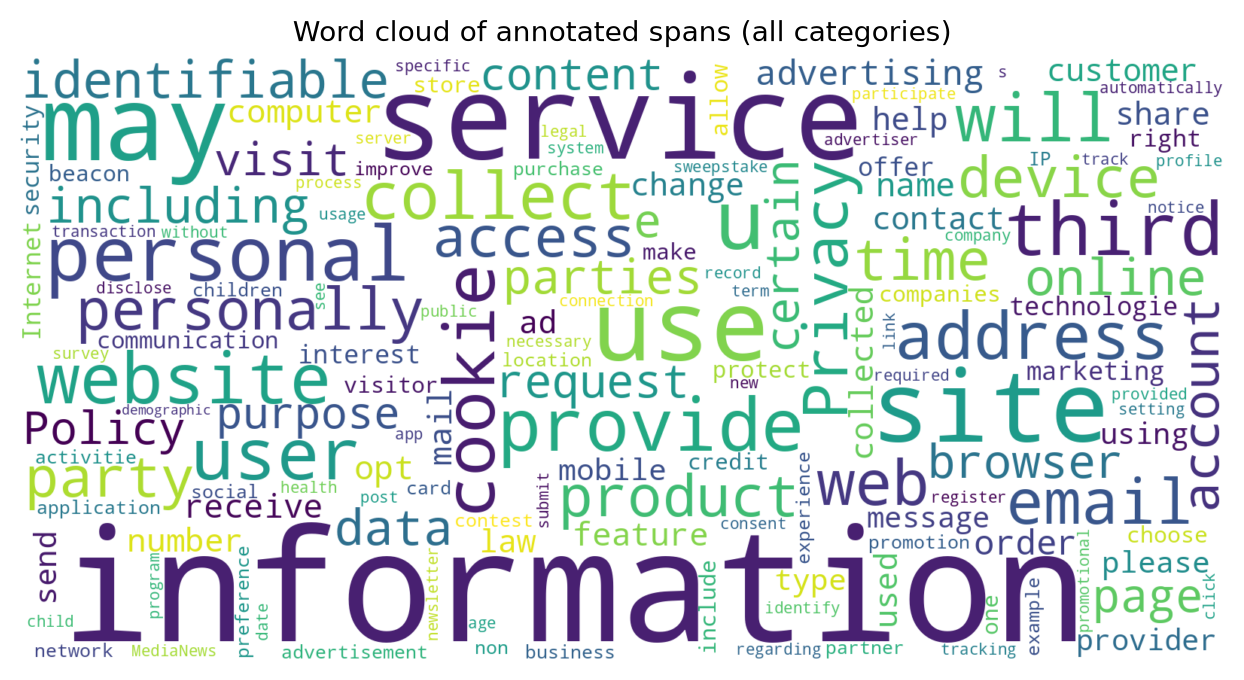
\includegraphics[width=\columnwidth]{figures/wordcloud.png}
\caption{Word cloud over all annotated spans (English stopwords removed).}
\label{fig:wordcloud}
\end{figure}

\subsection{Preprocessing}
\label{sec:preprocessing}

Rather than committing to a single fixed preprocessing pipeline, we define a
configurable text cleaner with five variants, each intended for a different downstream
representation, so that the effect of preprocessing choice can itself be compared
rather than assumed (as \S3.4 of the course specification requires). Every variant
first strips HTML markup inherited from the source policy pages and replaces URLs and
email addresses with placeholder tokens (\texttt{[URL]}, \texttt{[EMAIL]}) rather than
deleting them outright, so that the \emph{fact} that a policy names a contact mechanism
survives as signal for categories such as \emph{User Access, Edit and Deletion} while
the specific identity does not leak into the model as a feature -- consistent with our
decision to exclude policy and company identifiers from every generalization-focused
experiment. The five variants are: \textbf{base} (HTML removal, URL/email
substitution, lowercasing, whitespace normalization), intended for TF-IDF and the
classical models; \textbf{no\_stopwords} (base plus NLTK English stopword removal
\cite{bird-etal-2009-natural}), intended to sharpen content-word signal for TF-IDF;
\textbf{lemmatized} (base plus WordNet lemmatization), intended for the recurrent
neural models, where reducing surface-form sparsity shrinks the vocabulary the
embedding layer must learn from a comparatively small (${\sim}$11,000-row) training
split; \textbf{aggressive} (stopwords and lemmatization combined), intended for the
sparsest bag-of-words configurations; and \textbf{minimal} (HTML removal and
lowercasing only), intended for BERT Base, whose own WordPiece tokenizer and pretrained
attention mechanism are designed to make use of function words and surface context that
the more aggressive variants would discard. Lowercasing is applied uniformly because
the eight categories are distinguished by vocabulary and semantics rather than by
capitalization patterns. Figure~\ref{fig:preprocessing} compares the five variants on
the working corpus: stopword removal and lemmatization each shrink the vocabulary by
roughly a third relative to \textbf{base}, and combining them (\textbf{aggressive})
yields the smallest vocabulary and shortest mean span length of any variant, quantifying
the sparsity/information trade-off that motivates using different variants for different
downstream representations rather than a single fixed choice.

\begin{figure}[t]
\centering
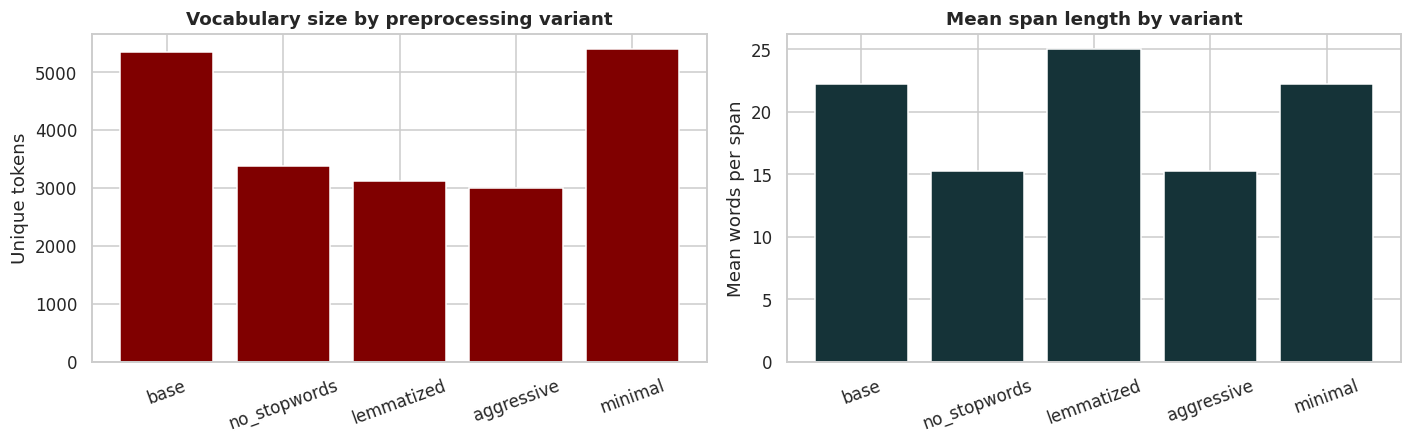
\includegraphics[width=\columnwidth]{figures/preprocessing_variants.png}
\caption{Vocabulary size and mean span length across the five preprocessing variants,
measured on a 3{,}000-span sample of the working corpus.}
\label{fig:preprocessing}
\end{figure}

\subsection{Word Representations}
\label{sec:representations}

The course specification requires at least two of TF-IDF, word2vec, and GloVe as
genuine text representations. Our design covers all three, described here as the
intended representation pipeline; the current empirical status of each is stated
precisely in Section~\ref{sec:results} rather than assumed.

\paragraph{TF-IDF.} A term frequency--inverse document frequency representation over the
\texttt{base}-preprocessed span, with a 5{,}000-term vocabulary, unigrams and bigrams,
minimum document frequency 5, maximum document frequency 0.8, sublinear term-frequency
scaling, and Unicode accent stripping \cite{pedregosa-etal-2011-scikit}. The vectorizer
is refit independently on the training portion of \emph{each} split scheme
(Section~\ref{sec:protocol}) rather than reused across schemes, since a vectorizer fit
once on a leaky split's vocabulary would itself leak information into the
policy-disjoint condition.

\paragraph{word2vec.} A skip-gram word2vec model \cite{mikolov-etal-2013-efficient},
implemented via \texttt{gensim} \cite{rehurek-sojka-2010-software} with 100-dimensional
embeddings, a context window of 5, and a minimum token count of 2, trained on the
project's own training-split vocabulary at a fixed random seed for reproducibility.
%TODO: this class is implemented but has not yet been executed in this environment
%(the gensim dependency is not currently installed); results depending on it are
%stubbed in Section~\ref{sec:results}.

\paragraph{GloVe.} A 100-dimensional GloVe representation \cite{pennington-etal-2014-glove},
either trained on the project's own corpus or initialized from publicly available
pretrained vectors, intended as a second, independently trained embedding baseline to
compare against word2vec's skip-gram objective.
%TODO: as with word2vec, this representation is implemented but not yet executed;
%see Section~\ref{sec:results} and the Limitations discussion in
%Section~\ref{sec:conclusion}.

\subsection{Model Architectures}
\label{sec:models}

\paragraph{Classical machine learning.} We train all three classical models required by
the course specification: Random Forest, (multinomial) Naive Bayes, and Logistic
Regression, each over the TF-IDF representation of Section~\ref{sec:representations},
using their \texttt{scikit-learn} implementations \cite{pedregosa-etal-2011-scikit}.
Each model is tuned over three hyperparameter configurations
(Table~\ref{tab:ml-grid}), selected on validation macro-F1, with only the winning
configuration scored on the held-out test set, following the manual-tuning protocol
required by the course specification (\S3.8).

\begin{table}[t]
\centering
\small
\begin{tabular}{@{}p{0.29\linewidth}p{0.62\linewidth}@{}}
\toprule
\textbf{Model} & \textbf{Configurations} \\
\midrule
Random Forest & 200 trees / unlimited depth; 400 trees / depth 60, min-split 5; 300
trees / depth 30, min-split 2, class-weighted \\
Logistic Regression & $C{=}1.0$; $C{=}5.0$; $C{=}1.0$, class-weighted (all
\texttt{lbfgs}, up to 2{,}000 iterations) \\
Naive Bayes & $\alpha{=}1.0$; $\alpha{=}0.3$; $\alpha{=}0.05$ \\
\bottomrule
\end{tabular}
\caption{Hyperparameter grids for the three classical models (3 configurations each,
2 split schemes -- 18 tuning runs total).}
\label{tab:ml-grid}
\end{table}

\paragraph{Recurrent neural networks.} We train all six required recurrent
architectures -- SimpleRNN, GRU \cite{cho-etal-2014-learning}, LSTM
\cite{hochreiter-schmidhuber-1997-lstm}, and their bidirectional counterparts
\cite{schuster-paliwal-1997-bidirectional} -- sharing one architecture family and
protocol: an embedding layer initialized from scratch, followed by a
(bidirectional) recurrent layer, dropout regularization, and a dense softmax
classification head over the eight categories, matching the architecture used in the
course's own reference notebooks. Input sequences use the \texttt{lemmatized}
preprocessing variant, are word-index-encoded from a vocabulary fit on the training
split only, and are padded or truncated to 48 tokens (Section~\ref{sec:dataset}).
Models are implemented in PyTorch \cite{paszke-etal-2019-pytorch} rather than
TensorFlow/Keras, since the interpreter used for this project (Python 3.14) has no
available TensorFlow distribution; the training objective (cross-entropy over integer
class labels) and architecture are otherwise unchanged from the reference formulation.
Each of the six models is tuned over three configurations (embedding dimension 64 or
128; hidden dimension 32 or 64; dropout 0.3 or 0.5; learning rate $5{\times}10^{-4}$ or
$10^{-3}$; one configuration per model additionally applies class-weighted loss),
selected on validation macro-F1 with early stopping (patience 3 epochs, maximum 12
epochs), for $3 \times 6 \times 2 = 36$ tuning runs across both split schemes.

\paragraph{BERT Base.} We fine-tune \texttt{bert-base-uncased}
\cite{devlin-etal-2019-bert} via the HuggingFace \texttt{transformers} library as the
seventh required neural model, using the \texttt{minimal} preprocessing variant so that
the model's own WordPiece tokenizer and pretrained attention mechanism see text as close
to its original form as possible. Because this project trains on consumer laptop
hardware (8\,GB RAM, Apple M2, no discrete GPU) rather than a datacenter accelerator, we
adopt a resource-constrained partial fine-tuning configuration rather than a full
fine-tune: the token embeddings and the first 10 of BERT's 12 encoder layers are
frozen, leaving only the final 2 encoder layers and the classification head trainable
(13.5\% of total parameters), and input sequences are truncated to 64 tokens (covering
the 90th percentile of span length) rather than the default 96--128. This follows
\citet{devlin-etal-2019-bert}'s own observation that most of BERT's task-specific
adaptation concentrates in its upper layers, and reduces training cost from an
estimated ${\sim}$40 minutes per epoch under full fine-tuning to approximately 2 minutes
per epoch, making the required six tuning runs (3 configurations $\times$ 2 split
schemes, varying learning rate, batch size, and one class-weighted configuration)
practical within the project's hardware and time budget. We report this constraint
explicitly rather than silently, and return to its consequences for the reported
numbers in Section~\ref{sec:results} and the Limitations discussion in
Section~\ref{sec:conclusion}.

\subsection{Split Schemes and Experimental Protocol}
\label{sec:protocol}

Every one of the ten models above is trained and evaluated identically under two split
schemes, both constructed at a fixed random seed for reproducibility.

\paragraph{\texttt{random}: row-level stratified split.} Rows are split
70/15/15 into train/validation/test, stratified by category, with no regard for which
policy or clause a row originates from. This is the leaky, optimistic condition that a
conventional classification pipeline -- including, notably, the course's own reference
notebooks -- would typically produce, and it is reported here \emph{only} as an explicit
point of comparison against the honest condition below, never as a standalone
generalization estimate.

\paragraph{\texttt{policy}: policy-disjoint split.} Policies, not rows, are the unit of
assignment: approximately 80\% of policies are assigned to training (further split into
train and validation by policy), and the remaining policies form a test set, such that
no policy's rows appear in more than one of the three sets. This is the paper's
generalization estimate, and is the scheme used for every model-selection and final
reported number outside of the explicit leakage comparison in
Section~\ref{sec:results}.

For every model and every scheme, model selection uses validation macro-F1, and only
the winning configuration is evaluated on the held-out test set, so that the number of
configurations tried never itself inflates the reported test score. Every model report
includes accuracy, macro-F1, weighted-F1, full per-class precision/recall/F1, and a
confusion matrix, consistent with the evaluation requirements of the course
specification (\S3.9).

\section{Results}
\label{sec:results}

All three required classical models and all seven required neural models were trained
and evaluated to completion under both split schemes described in
Section~\ref{sec:protocol}, for a combined 60 logged tuning runs (18 classical, 36
recurrent, 6 BERT Base). All numbers below are drawn directly from the executed project
notebook (\texttt{project\_440.ipynb}) rather than recomputed for this paper.

\subsection{Model Comparison}
\label{sec:model-comparison}

Table~\ref{tab:comparison} reports test-set performance for every model's
best validated configuration under both split schemes, and
Figure~\ref{fig:comparison} visualizes the same comparison, ranked by policy-disjoint
macro-F1.

\begin{table*}[t]
\centering
\small
\begin{tabular}{@{}llrrr@{}}
\toprule
\textbf{Scheme} & \textbf{Model} & \textbf{Accuracy} & \textbf{Macro-F1} & \textbf{Weighted-F1} \\
\midrule
random & Logistic Regression & 0.7740 & \textbf{0.7534} & 0.7713 \\
random & Naive Bayes & 0.7575 & 0.7258 & 0.7547 \\
random & Random Forest & \textbf{0.7798} & 0.7212 & 0.7739 \\
random & BERT Base & 0.7586 & 0.7208 & 0.7553 \\
random & Bidirectional GRU & 0.7640 & 0.6999 & 0.7611 \\
random & Bidirectional LSTM & 0.7598 & 0.6840 & 0.7568 \\
random & Bidirectional SimpleRNN & 0.7283 & 0.6118 & 0.7222 \\
random & LSTM & 0.6914 & 0.5489 & 0.6826 \\
random & GRU & 0.7110 & 0.5194 & 0.7043 \\
random & SimpleRNN & 0.4823 & 0.1719 & 0.4080 \\
\midrule
policy & \textbf{BERT Base} & 0.7152 & \textbf{0.7060} & 0.7138 \\
policy & Naive Bayes & \textbf{0.7026} & 0.7011 & 0.6987 \\
policy & Logistic Regression & 0.6789 & 0.6923 & 0.6770 \\
policy & Random Forest & 0.6771 & 0.6516 & 0.6673 \\
policy & Bidirectional LSTM & 0.6699 & 0.6083 & 0.6663 \\
policy & Bidirectional GRU & 0.6331 & 0.5859 & 0.6344 \\
policy & Bidirectional SimpleRNN & 0.6175 & 0.4891 & 0.6090 \\
policy & GRU & 0.5850 & 0.4755 & 0.5832 \\
policy & LSTM & 0.5794 & 0.4425 & 0.5764 \\
policy & SimpleRNN & 0.3863 & 0.1310 & 0.3357 \\
\bottomrule
\end{tabular}
\caption{Test performance at each model's best validated configuration under both
split schemes, ranked by macro-F1 within each scheme. Bold marks the best value in
each column within each scheme.}
\label{tab:comparison}
\end{table*}

\begin{figure}[t]
\centering
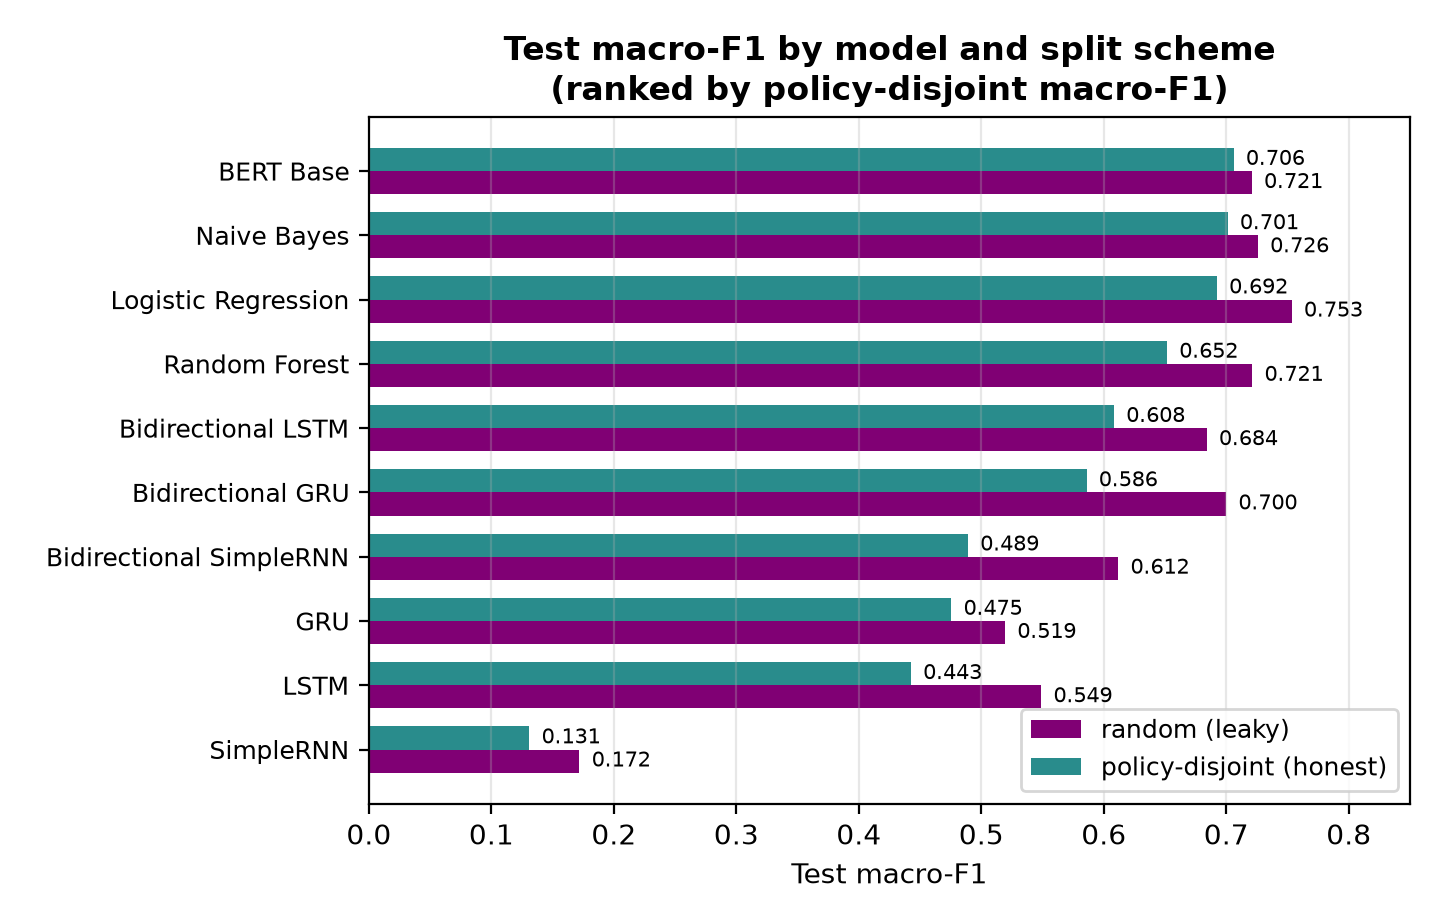
\includegraphics[width=\columnwidth]{figures/model_comparison.png}
\caption{Test macro-F1 for all ten models under both split schemes, ranked by
policy-disjoint (honest) macro-F1.}
\label{fig:comparison}
\end{figure}

Under the honest, policy-disjoint scheme, \textbf{BERT Base} attains the best overall
macro-F1 (0.7060), narrowly ahead of a tuned Naive Bayes classifier (0.7011) -- a
0.0049 gap close enough that the two should be read as near-tied rather than a decisive
win. \textbf{SimpleRNN} is the worst model overall (macro-F1 0.1310, barely above what a
majority-class-only baseline would score, $\approx$0.08), and \textbf{Random Forest} is
the worst classical model (macro-F1 0.6516). Under the leaky \texttt{random} scheme, by
contrast, Logistic Regression appears to lead (0.7534) and BERT Base falls to fourth
place, barely ahead of Bidirectional GRU (0.7208 vs.\ 0.6999) and behind two classical
models it beats decisively under the honest scheme -- a direct illustration of why a
single split scheme is an unreliable basis for declaring a winner, echoing the broader
evaluation-methodology concern raised by \citet{gorman-bedrick-2019-need}.

A concrete instance of the accuracy trap motivating our macro-F1-first protocol appears
within the classical models alone: under the leaky split, Random Forest has the
\emph{highest} accuracy of all ten models (0.7798) while having the \emph{lowest}
macro-F1 of the three classical models (0.7212), because unpruned trees can memorize the
47\%-majority class's boilerplate phrasing without penalty under an accuracy metric. A
project selecting by accuracy on a conventional split would ship this model, its worst
classical generalizer.

\subsection{The Effect of Leakage}
\label{sec:leakage}

Figure~\ref{fig:leakage} shows, for every model, the macro-F1 inflation between the
leaky \texttt{random} scheme and the honest \texttt{policy}-disjoint scheme.

\begin{figure}[t]
\centering
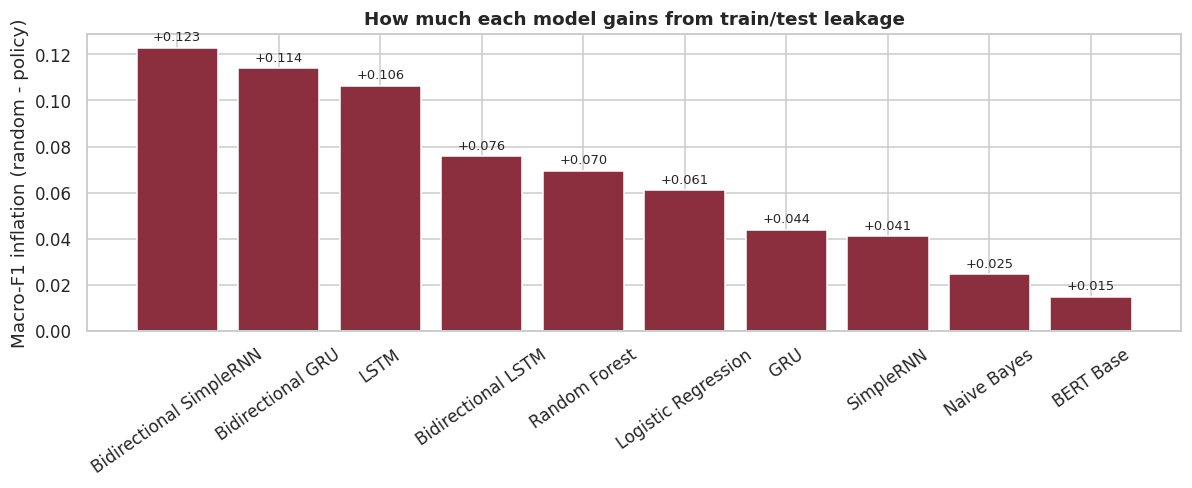
\includegraphics[width=\columnwidth]{figures/leakage_inflation.png}
\caption{Macro-F1 inflation (random-split score minus policy-disjoint score) by model.
Larger bars indicate a model whose apparent performance depends more heavily on
memorizing boilerplate text shared across the leaky split's train and test sets.}
\label{fig:leakage}
\end{figure}

Evaluating on the row-level split overstates macro-F1 by between +0.015 (BERT Base) and
+0.123 (Bidirectional SimpleRNN) depending on model. The inflation is not explained by
any single structural property: directionality alone does not predict it, since
Bidirectional SimpleRNN (+0.123) and Bidirectional GRU (+0.114) inflate \emph{more} than
their unidirectional counterparts (+0.041 and +0.044), while unidirectional LSTM
(+0.106) inflates \emph{more} than Bidirectional LSTM (+0.076) -- the opposite pattern.
What is consistent is architecture family and the extremes. The three classical models
and BERT Base form a tight, low-inflation cluster (+0.015 to +0.070); the six recurrent
architectures, trained from scratch on this project's own ${\sim}$12,000 training spans
with no external pretraining to fall back on, show both the highest and the most
variable inflation (+0.041 to +0.123), with three of six gaining more than +0.10
macro-F1 purely from the leaky split -- Bidirectional GRU, Bidirectional SimpleRNN, and
unidirectional LSTM. \textbf{BERT Base shows the smallest inflation of any model
trained} (+0.0148 macro-F1), consistent with the interpretation that a pretrained
transformer's representations, learned from a vastly larger and more diverse external
corpus than this project's training spans, rely comparatively less on memorizing this
dataset's specific boilerplate phrasing; \textbf{Naive Bayes is the only other model
under +0.03} (+0.0247), plausibly because its conditional-independence assumption
learns per-token, per-class frequencies that are largely insensitive to which specific
policy a token happened to appear in. SimpleRNN's own inflation is modest in absolute
terms (+0.041) largely because its macro-F1 is so low under either scheme (0.13--0.17)
that there is little score left to inflate -- a ceiling effect rather than evidence of
memorization-resistance, and a reminder that raw inflation should be read alongside
absolute performance, not in isolation. Taken together with the accuracy trap in
Section~\ref{sec:model-comparison}, this is this project's central methodological
finding: a conventional stratified split, scored on accuracy or even on an unexamined
single-split macro-F1, would have led this project to select one of its
worst-generalizing models -- and it would have done so silently, since nothing about
the leaky split's numbers alone reveals the problem.

\subsection{Per-Class Performance of the Best Model}
\label{sec:per-class}

Table~\ref{tab:perclass} reports per-class precision, recall, and F1 for BERT Base
under the policy-disjoint test set. BERT Base's own confusion matrix was not among this
run's saved outputs, so Figure~\ref{fig:confusion} instead shows the row-level confusion
matrices for the three classical models on the same policy-disjoint test set -- real,
directly plotted output rather than a reconstruction, and the natural companion to
Table~\ref{tab:perclass} since Naive Bayes (Section~\ref{sec:model-comparison}) is
BERT's closest competitor on this split.

\begin{table}[t]
\centering
\small
\begin{tabular}{@{}lrrr@{}}
\toprule
\textbf{Category} & \textbf{P} & \textbf{R} & \textbf{F1} \\
\midrule
Intl.\ \& Specific Audiences & 0.86 & 0.88 & \textbf{0.87} \\
Policy Change & 0.91 & 0.77 & 0.84 \\
Data Security & 0.77 & 0.88 & 0.82 \\
First Party Collection/Use & 0.76 & 0.78 & 0.77 \\
Third Party Sharing/Collection & 0.66 & 0.64 & 0.65 \\
User Access, Edit \& Deletion & 0.69 & 0.57 & 0.62 \\
User Choice/Control & 0.56 & 0.62 & 0.59 \\
Data Retention & 0.86 & 0.35 & \textbf{0.49} \\
\bottomrule
\end{tabular}
\caption{Per-class precision, recall, and F1 for BERT Base on the policy-disjoint test
set (overall accuracy 0.7152, macro-F1 0.7060).}
\label{tab:perclass}
\end{table}

\begin{figure*}[t]
\centering
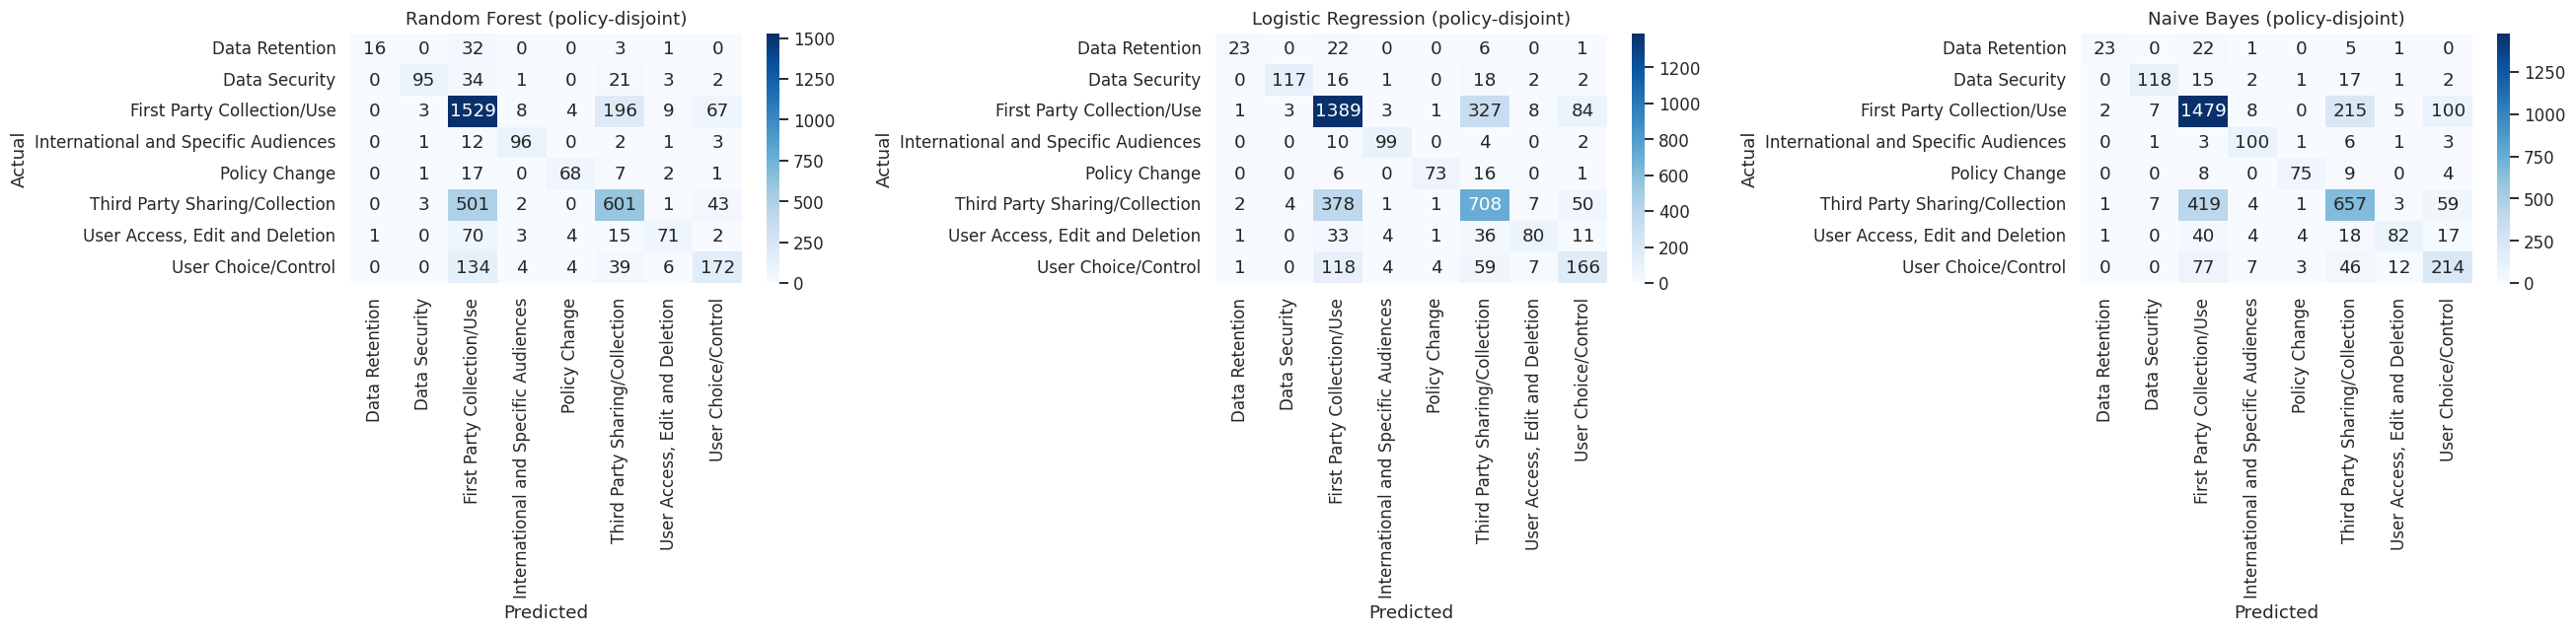
\includegraphics[width=\textwidth]{figures/confusion_matrices_classical.png}
\caption{Confusion matrices for the three classical models on the policy-disjoint test
set. All three show the same dominant error mode: confusion between \emph{First Party
Collection/Use} and \emph{Third Party Sharing/Collection}.}
\label{fig:confusion}
\end{figure*}

Class size is a poor predictor of per-class difficulty (correlation between dataset
class count and per-class F1 measured at approximately +0.05, effectively no
relationship): \emph{Policy Change} and \emph{International and Specific Audiences} are
among the smallest categories in the dataset yet score highest, because both use
distinctive, formulaic vocabulary (``\emph{we may update this policy from time to
time}''; ``\emph{residents of the European Economic Area}'') that a model needs
comparatively few examples to learn. Figure~\ref{fig:confusion} shows that the dominant
error mode for every classical model is \emph{semantic overlap} between \emph{First
Party Collection/Use} and \emph{Third Party Sharing/Collection}, which describe the same
underlying act -- data collection -- and differ chiefly in \emph{who} receives the data,
a distinction sometimes carried by a single noun phrase within a 22-word span (e.g.\
Naive Bayes misclassifies 419 of 1{,}151 \emph{Third Party Sharing/Collection} test rows
as \emph{First Party Collection/Use}, and 215 of 1{,}816 \emph{First Party
Collection/Use} rows the other way). Table~\ref{tab:perclass} shows the same
pattern persists under BERT's pretrained representation: \emph{First Party
Collection/Use} and \emph{Third Party Sharing/Collection} are its two weakest categories
among the frequent classes (F1 0.77 and 0.65) despite having by far the most training
examples, while the small-but-distinctive categories all reach F1 0.82 or higher. \emph{Data
Retention}, by contrast, is the one category where scarcity does appear to be the
bottleneck: its precision is high (0.86) but recall is the lowest of any category
(0.35), consistent with a model that recognizes the category correctly when it commits
to it but has too few training examples to recognize it reliably in the first place.

\subsection{Representation and Resource Constraints}
\label{sec:constraints}

%TODO: the word2vec and GloVe representations described in Section~\ref{sec:representations}
%have not yet been executed in this environment (the required \texttt{gensim} dependency
%is not currently installed), so all results above use only the TF-IDF representation for
%the classical models. Installing \texttt{gensim} and executing both representation
%classes on the training split of each scheme is required to satisfy the course's
%at-least-two-representations requirement and will be added here once complete.

%TODO: the BERT Base numbers reported above come from a resource-constrained partial
%fine-tune (Section~\ref{sec:models}: embeddings + bottom 10 of 12 encoder layers
%frozen), not a full fine-tune. A full, non-frozen-layer fine-tune (given GPU access) is
%planned to quantify how much headroom the frozen layers cost; no such run has been
%executed yet, so no specific number is claimed here.

\section{Conclusion}
\label{sec:conclusion}

We presented a leakage-aware evaluation of privacy-practice classification on the
OPP-115 corpus, training and evaluating three classical machine learning models and
seven neural architectures -- spanning bag-of-words classifiers, recurrent networks,
their bidirectional variants, and a fine-tuned transformer -- under both a conventional
row-level split and a policy-disjoint split that respects the document-level structure
of the data. The central finding is that these two evaluation conditions do not just
differ in absolute score, they disagree about which model is best: a conventional split
rewards models with the raw capacity to memorize boilerplate legal language -- most
visibly Bidirectional SimpleRNN, Bidirectional GRU, and unidirectional LSTM, each
gaining more than +0.10 macro-F1 purely from the leaky split -- while several of these
same models rank near the bottom under honest evaluation. Under policy-disjoint
evaluation, a resource-constrained fine-tune of BERT Base is the strongest model
(macro-F1 0.7060), and it is also the least inflated by leakage of any model trained
(+0.0148) -- consistent with the interpretation that its advantage comes from
pretraining on external data rather than from memorizing this corpus specifically. We
take this as evidence that leakage-aware, document-grouped evaluation is not a niche
concern specific to this dataset, but a methodological practice that any text
classification project built on documents with reused, template-like language --
contracts, terms of service, regulatory filings, form letters -- should adopt by
default. As stated in Section~\ref{sec:intro}, we treat this single, fully executed
protocol as this paper's whole novelty claim, deliberately leaving the three related
directions below as designed-but-unrun future work rather than diluting this claim
across several partial ones.

\paragraph{Limitations.} This work has several limitations that should be read
alongside the numbers above. First, only TF-IDF is currently a genuinely executed
representation; the word2vec and GloVe representations described in
Section~\ref{sec:representations} are implemented but have not yet been run to
completion in this environment (Section~\ref{sec:constraints}). Second, the reported
BERT Base numbers come from a partial, layer-frozen fine-tune constrained by consumer
hardware rather than a full fine-tune (Section~\ref{sec:models}); a full, non-frozen-layer
fine-tune, not yet attempted, may leave real headroom above the reported figures. Third,
all results in this paper are
\emph{oracle-span}: the dataset supplies the relevant span directly, so a deployed
system would additionally require an upstream step to identify which spans of a raw
policy document are worth classifying at all, which this work does not address. Fourth,
the policy-disjoint validation set is a single fixed-seed policy-level draw rather than
a cross-validated estimate over multiple policy folds, so its precision should not be
over-interpreted. Finally, provenance metadata for consolidation rows produced by
merging two or three annotators' judgments is approximate rather than exact
(the corpus's released files do not retain which raw annotations fed a given merge), so
any future experiment that weights training examples by annotator agreement inherits
this uncertainty.

\paragraph{Future work.} Four directions follow directly from the findings above and
from the scoped-out brainstorming directions named in Section~\ref{sec:intro}. First,
the 34.9\% of clauses that legitimately carry multiple categories
(Section~\ref{sec:dataset}) suggest that feeding span-plus-clause context, rather than
the span alone, should specifically help disambiguate the First-Party/Third-Party
confusion identified as the dominant error mode in Section~\ref{sec:per-class}, since
the distinguishing noun phrase for that pair often sits just outside the annotated
span. Second, because Section~\ref{sec:per-class} shows that class size is a poor
predictor of per-class difficulty and that the dominant failure mode is semantic overlap
rather than scarcity, minority-class-aware training strategies (class weighting, focal
loss, balanced sampling) are expected to help the one class where scarcity does appear
to bite -- \emph{Data Retention} -- more than they help the semantically overlapping,
already-frequent \emph{Third Party Sharing/Collection} category. Third, the external
validation study scoped out in Section~\ref{sec:intro} would apply this paper's best
model (BERT Base, chosen both for its top honest-scheme macro-F1 and its smallest
leakage inflation) to a different market of English-language privacy policies to test
whether a classifier trained purely on OPP-115's US-policy distribution transfers;
any resulting disclosure or risk comparison would need to stay a descriptive NLP
finding, never a compliance or legal judgment about a named company. Fourth, closing the
two gaps
identified in the Limitations paragraph -- executing the word2vec and GloVe
representations, and attempting a full, non-frozen-layer BERT fine-tune given access to
GPU resources -- would let this project's reported numbers be read as closer to each
method's ceiling rather than a hardware-constrained lower bound.

\bibliography{custom}
\bibliographystyle{acl_natbib}

\end{document}
